% !TeX program = xelatex
% !TeX encoding = utf-8
% 《机器人》LaTeX模板
% 面向往复夹持递送的血管介入机器人力反馈扰动建模与残差抑制

\documentclass{JQRnew}

\JQRsetup{
 % 期刊出版信息
 volume     = xx,
 number     = x,
 year       = 2026,
 month      = 10,
 doi        = 240001,
 % 基金项目
 funds      = {国家自然科学基金联合基金项目（U23A20338）；国家重点研发计划智能机器人重点专项（2022YFB4703500）；辽宁省自然科学基金优青项目（2023-MS-021）},
 % 通信作者
 corrauthor = {刘浩，Email: liuhao@sia.cn},
 % 日期
 dates      = {2026-10-21/2026-10-21/2026-10-21},
 %
 % ---- 中文相关信息
 cntitle    = {面向往复夹持递送的血管介入机器人力反馈扰动建模与残差抑制},
 cnauthor   = {隋凯丞\addr{1,2,3}, 郑力铭\addr{1,2,3}, 林\quad 鹏\addr{1,2}, 胡琨元\addr{1,2*}, 刘\quad 浩\addr{1,2*}},
 runtitle   = {隋凯丞，等：面向往复夹持递送的血管介入机器人力反馈扰动建模与残差抑制},
 cnaddress  = {1. 中国科学院沈阳自动化研究所 机器人学国家重点实验室，辽宁~~沈阳\quad 110016；\\
               2. 辽宁省微创手术机器人重点实验室，辽宁~~沈阳\quad 110016；\\
               3. 中国科学院大学，北京\quad 100049},
 %
 % ----- 中文摘要
 cnabstract = {【目的】针对夹持式血管介入机器人典型的往复运动引起的附加测力波动，研究力反馈扰动建模与补偿方法，重构相同递送条件下不发生夹爪换手时的连续力反馈。【方法】将主副夹爪的递送、交接、回程和重夹持过程划分为十个阶段，建立浮动传力组件的惯性干扰模型与多级串联刚度模型；采用轴向与周向耦合的等效恢复行程，计算重加载实际承载与连续递送目标之间的补偿量，并将物理模型输出、换手前稳态载荷、相对运动与夹爪时序输入门控循环单元（GRU）网络，学习物理模型难以标定的参数，估计物理模型输出与连续递送运动下力觉之间的残差；通过交接期数值锁存与边界平滑输出反馈力和扭矩。【结果】以不换手递送试次作为连续载荷参考，评价稳态与重加载阶段的反馈重构误差、完整交接重加载周期的输出波动及S1/S9阶段的未训练阻力突变响应，并在介入血管模型中验证受压推进与旋转递送的反馈波形。重构误差、最大波动及扰动响应结果为[待补]。【结论】物理模型与GRU残差补偿相结合，为往复夹持递送中的连续力反馈重构提供了方法。},
 % ---- 中文关键字
 cnkeywords = {导丝；介入机器人；夹持机构；接触力学；扭矩传递；力反馈；GRU神经网络},
 %
 % ---- 英文相关信息
 entitle    = {Disturbance Modeling and Residual Suppression of Force Feedback for Vascular Intervention Robot in Reciprocating Clamping Delivery},
 enauthor   = {SUI Kaicheng\addr{1,2,3}, LIN Peng\addr{1,2}, WANG Chongyang\addr{1,2}, ZHANG Yuhang\addr{1,2}, PAN Pengyu\addr{4}, LIU Hao\addr{1,2*}},
 enaddress  = {1. \textit{State Key Laboratory of Robotics, Shenyang Institute of Automation, Chinese Academy of Sciences, Shenyang} 110016, \textit{China}; \\
               2. \textit{Key Laboratory of Minimally Invasive Surgical Robot, Liaoning Province, Shenyang} 110016, \textit{China}; \\
               3. \textit{University of Chinese Academy of Sciences, Beijing} 100049, \textit{China}},
 %
 % ---- 英文摘要
 enabstract = {[Objective] A disturbance model and residual compensation method are developed to reconstruct the continuous force feedback expected without gripper handover under matched delivery conditions in a reciprocating clamping vascular intervention robot. [Methods] The delivery, handover, return, and reclamping cycle is divided into ten stages (S1--S10). An inertial disturbance model of the floating load transmission assembly and a series stiffness model are established. A coupled axial-rotational recovery travel is used to calculate the compensation between the actual reloading load and the continuous-delivery target. The physical baseline, stored steady load before handover, relative motion, and gripper timing are supplied to a gated recurrent unit (GRU) network to estimate the residual relative to a continuous-delivery reference. Numerical holding during handover and boundary smoothing are applied to the force and torque feedback. [Results] Uninterrupted delivery trials on a coaxial tensile and torsional test rig provide the continuous-load reference for evaluating feedback reconstruction errors during steady delivery and reloading, output fluctuations over the complete handover and reloading cycle, and responses to untrained resistance changes in S1 and S9. Feedback waveforms are also examined during compressive delivery and rotation in a vascular phantom. Reconstruction errors, maximum fluctuations, and disturbance response results are [to be added]. [Conclusions] Combining the physical model with GRU residual compensation provides a method for reconstructing continuous force feedback during reciprocating clamping delivery.},
 %
 % ---- 英文关键字
 enkeywords = {guidewire; intervention robot; clamping mechanism; contact mechanics; torque transmission; force feedback; gated recurrent unit (GRU)}
}

% ----- 加载宏包
\usepackage{algorithm}
\usepackage{algpseudocode}
\usepackage{pifont}
\usepackage{balance}
\usepackage{mwe}
\usepackage{booktabs}
\usepackage{amsmath,amssymb}
\usepackage{bm}

\floatname{algorithm}{算法}
\renewcommand{\algorithmicrequire}{\textbf{输入:}}
\renewcommand{\algorithmicensure}{\textbf{输出:}}
\newcommand{\algorithmicchushi}{\textbf{初始化:}}

\begin{document}

\maketitle

% 引言部分不设节标题（遵循《机器人》期刊约定）
血管内介入治疗是实现心血管及脑血管疾病微创诊治的重要手段。在传统手术中，医师需在X射线透视引导下手动推进并旋转导丝与导管，这一过程不仅高度依赖术者的精准操作技巧与临床经验，还使术者长期暴露于电离辐射并承受沉重的铅衣负担\ucite{ref1}。血管介入机器人通过主从遥操作模式驱动柔性器械完成递送与旋转，可将术者与辐射源物理隔离，并提供高精度的可重复运动轨迹。然而，主从遥操作隔绝了术者与器械的直接物理接触，器械在血管内的受力状态必须经过从端测量与主端再现才能传递至术者\ucite{ref2}。因此，在测量器械操作载荷的基础上形成连续、清晰的主端力反馈，是帮助术者判断器械受阻状态的重要环节。

介入器械的力感知方案主要分为体内远端测力和体外近端测力两类，二者反映不同空间尺度的受力信息。远端测力将光纤布拉格光栅（FBG）等微型传感元件集成于器械尖端以直接感知末端接触力\ucite{ref3}，但受限于微细器械尺寸与封装工艺，制造成本高且难以兼容常规一次性耗材。相比之下，近端测力在体外驱动端通过传力路径中的力传感器\ucite{ref4,ref6}或驱动电机电流\ucite{ref5}获取沿器械传递的综合操作阻力，无需改造常规器械且便于无菌分离，但近端测力通道与机械驱动过程紧密耦合，器械真实负载与传动机构自身的运行干扰将同时作用于测量信号。

器械与驱动机构的接触方式决定了近端传力特性。滚轮摩擦驱动需维持法向预紧力，在推进与旋转复合运动时还会受到界面微滑移的影响\ucite{ref5}；仿人手往复夹持机构则通过面接触建立静摩擦连接\ucite{ref7}，便于控制夹紧力，并分别测量轴向递送力与周向旋转扭矩\ucite{ref8}。受直线导轨行程限制，此类机构通过主、副夹爪“夹持递送---释放回退---重新夹持”的周期性往复运动实现长距离输送\ucite{ref9,ref10}。对于承担近端测力功能的移动主爪，往复加减速引起的浮动组件惯性、旋转支路摩擦及夹爪接触切换会改变测力支路的受力平衡，造成反馈波动。

针对近端测量中的机构附加干扰分量，现有研究主要从运行偏置标定、动力学模型补偿及数据驱动估计等方面展开。在机理建模与标定方面，Sankaran等\ucite{ref5}在不同转速下采集机构自由递送时的空载电流，建立运行偏置与转速的映射关系并从总力中予以扣除。Bao等\ucite{ref8}综合分析了摩擦、重力及旋转速度对测量结果的影响，构建了基于载荷与转速的动态补偿模型，并在时变加载实验中验证了其相较于静态零偏补偿的优势。Wang等\ucite{ref12}建立了递送机构的平移与旋转动力学模型，结合运动学测量实时修正测力基线，并对扭矩信号的抖动进行了滤波处理。在数据驱动建模方面，时序神经网络为表征夹持与传力过程中的复杂非线性关系提供了有效途径。Lyu等\ucite{ref13}将机器人运动状态、夹持间距与软体夹持器的视觉形变序列输入长短期记忆网络（LSTM），实现了器械操作力与扭矩的端到端估计；Wang等\ucite{ref14}采用时间卷积网络（TCN）建立了近端测量与导丝远端接触力之间的时序映射关系。

上述研究分别讨论了运行偏置校正、连续运动补偿和时序力估计，但往复夹持递送还包含主副夹爪交替承载。载荷交接、回程启停惯性以及柔顺接触的变形重建与微滑移，会与真实血管阻力变化同时出现在近端测量信号中，形成卸载台阶和附加波动。因此，需要根据往复夹持的传力过程重构连续递送时的反馈载荷，在减小换手波动的同时保留有效承载阶段新增的血管阻力变化。

\section{问题描述（Problem description）}

\subsection{往复夹持递送过程}

本文研究的夹持式血管介入机器人采用主、副双夹爪交替夹持器械，通过夹爪与器械表面的摩擦接触传递运动和载荷。主夹爪安装于沿直线导轨移动的滑台上，负责器械的轴向推进与周向旋转，其内部集成轴向与周向两路传感器，用于在驱动器械的同时同步感知轴向递送力与周向旋转扭矩；副夹爪安装于近血管鞘入口端，用于在主夹爪松开与回退期间固定器械位置并承接血管端负载。

一般情况下夹持式的接入机器人进行的周期性短行程往复运动，根据控制时序与接触状态，可以分成S1～S10十个阶段，按操作过程归为以下四类（如图\ref{fig1}所示）：
\begin{enumerate}
\item[1)] 稳态递送相（S1～S2）：主爪独立夹持导丝推进与旋转（S1），单次行程结束时滑台制动停止而副爪尚未闭合（S2）；
\item[2)] 卸载交接相（S3～S4）：副爪闭合建立第一次双爪共持（S3），随后主爪释放导丝并将管腔负载转移至副爪（S4）；
\item[3)] 空载回程相（S5～S6）：主爪完全脱离导丝后沿导轨高速退回（S5）并在起点制动停止（S6），期间导丝由副爪独立固定；
\item[4)] 重加载交接相（S7～S9）与稳态恢复（S10）：主爪在起点重新闭合形成第二次双爪共持（S7），副爪释放导丝（S8），随后主爪带动导丝恢复向前推进，串联柔顺传力变形逐步重建、测力响应随载荷接管而动态爬升（S9）；当重夹持后的有效推进位移达到稳定承载阈值时重加载完成，主爪恢复独立稳态承载（S10，归入稳态递送相）并进入下一周期。
\end{enumerate}

\begin{figure*}[h!t]
	\centering
	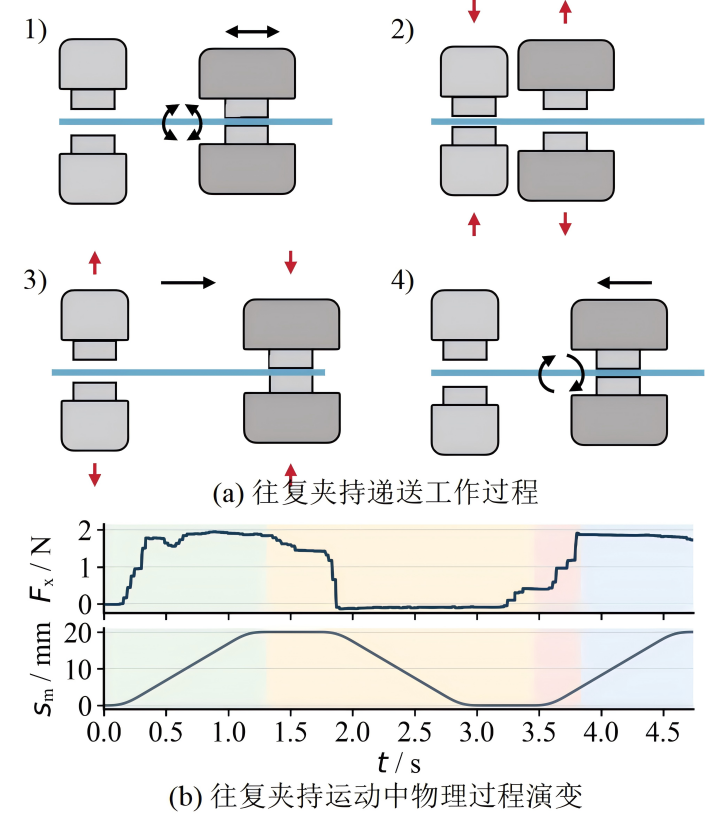
\includegraphics[width=0.88\linewidth]{fig1.png}
	\bicaption{往复夹持递送工作过程}{Timing of S1--S10 stages and evolution of physical phases during reciprocating clamping delivery}
	\label{fig1}
\end{figure*}

\subsection{测力波动与补偿目标}

在往复工作循环中，主夹爪交替经历承载推进与空载回退，机构运动与夹爪切换引起的附加干扰随阶段变化。主夹爪释放时，载荷向副爪转移，主爪测力支路发生阶跃卸载；快速回退时，随滑台运动的内侧浮动组件产生轴向惯性力；存在旋转运动时，旋转支路还受到惯性、轴承摩擦与阻尼的影响。重新夹持时的机械冲击，以及恢复推进初期柔顺支路的变形重建，会分别造成短暂波动和逐步恢复的测力响应。若直接将这些变化反馈至主端，术者会感受到周期性换手脉冲，影响对远端血管阻力的判断。

本文以相同初始受力状态、血管条件及有效推进与旋转轨迹下，主爪持续夹持器械时的连续递送载荷作为反馈目标。补偿量根据同步采集的运动状态、测力信号与夹持动作时序在线计算：在正常承载阶段扣除机构运动干扰，在S4～S8期间锁存换手前的反馈值，在S9期间根据实际承载与变形恢复过程重构连续递送反馈，并保留实时测力通道对新增阻力和阻力矩的响应。

全文设轴向正方向沿导丝名义中心轴指向远端血管，旋转角正方向遵循右手定则，分别采用 ${\rm N}$、${\rm N}\cdot{\rm mm}$、${\rm mm}$、${\rm rad}$ 和 ${\rm s}$ 作为力、扭矩、位移、角位移和时间的单位。主爪原始测量的轴向力记为 $F_{xm}$，绕器械轴线的测量扭矩记为 $\tau_{xm}$；扭矩可由扭矩传感器直接测得，也可由切向力经标定力臂换算。补偿后的主端力与扭矩反馈量分别记为 $F_{xc}$ 和 $\tau_{xc}$。

\subsection{本文工作}

围绕往复夹持递送过程中的近端测力波动抑制问题，本文开展以下三方面研究工作：
\begin{enumerate}
\item[1)] 多阶段传力建模：分析主副夹爪交替承载的传力过程，建立正常递送、双爪交接与重加载阶段的动力学和串联接触刚度模型。
\item[2)] 物理模型与GRU时序残差补偿方法构建：建立扣除机构运动干扰并包含二维重加载过渡项的物理动力学模型，结合换手前稳态载荷锁存与边界平滑；引入GRU网络利用历史运动与时序特征在线估计物理模型与连续递送参考之间的残差，降低未建模微滑移与接触迟滞的影响。
\item[3)] 参数辨识与实验评估：通过实验台辨识物理参数，定量评价连续力反馈重构误差、换手全周期波动及突发阻力响应，并通过消融实验分析重加载模型与残差学习的贡献；在介入血管模型中验证模型扰动消除能力。
\end{enumerate}

本文其余部分组织如下：第2节建立多阶段传力模型、重加载物理过渡项与融合机理规律的GRU时序残差补偿方法；第3节开展同轴参考定量评估、未训练扰动测试与血管模型递送实验；第4节与第5节分别给出讨论与结论。

\section{往复夹持传力机理与残差补偿方法（Reciprocating clamping transmission mechanism and residual compensation method）}

本节围绕主、副夹爪交替承载过程，建立远端血管阻力、夹持界面传力与近端测量读数之间的关系。通过分析正常递送、双爪载荷交接及重加载过程中的轴向与旋转耦合，确定连续递送载荷与机构附加干扰项，为后续物理模型与时序残差补偿提供依据。

\subsection{递送测量关系与交接载荷分配}

对主、副夹爪共同作用的受载系统应用准静态平衡条件，忽略器械质量与分布摩擦，沿器械轴线的轴向力与绕轴扭矩满足：
\begin{align}
	\label{eq1}
	\begin{cases}
		F_{M} + F_{S} = F_{\text{out}}, \\
		\tau_{M} + \tau_{S} = \tau_{\text{out}}
	\end{cases}
\end{align}
式中，$F_{\text{out}}$ 与 $\tau_{\text{out}}$ 分别为远端血管对器械施加的轴向阻力与阻力矩，以阻碍推进和正转为正方向；$F_M$、$\tau_M$ 与 $F_S$、$\tau_S$ 分别为主、副夹爪施加于器械的轴向力与扭矩。定义连续递送的目标载荷向量 $\bm{w}_{\text{cont}} = [F_{\text{cont}},\tau_{\text{cont}}]^{\rm T}$，主、副爪载荷向量分别为 $\bm{w}_M = [F_M,\tau_M]^{\rm T}$ 与 $\bm{w}_S = [F_S,\tau_S]^{\rm T}$。在单爪独立承载的稳态递送阶段，副爪完全松开，$F_S = \tau_S = 0$，外载由主爪单独平衡，即 $\bm{w}_M = \bm{w}_{\text{out}}$。

测力传感器一般安装在浮动传力组件与滑台间，随滑台平移并随旋转机构转动，传感器原始测量向量除包含器械接触载荷外，还叠加了运动部件的动力学干扰与零位偏置：
\begin{align}
	\label{eq2}
	\bm{y} &= \bm{H}_{0}\bm{w}_{M} + \bm{d} + \bm{\varepsilon},\quad \bm{d} = \bm{p}(\bm{q}_{M},\bm{c}) + \bm{b} \\
	\label{eq3}
	\bm{p}(\bm{q}_{M},\bm{c}) &=
	\begin{bmatrix}
		m_s a_M \\
		J_s\alpha_M
	\end{bmatrix}
	+ \bm{p}_{\text{clamp}}(\bm{c})
\end{align}
式中，$\bm{H}_0$ 为离线标定的传递矩阵；$\bm{b}$ 为静态零偏；$\bm{\varepsilon}$ 为测量噪声；$a_M$ 和 $\alpha_M$ 为主爪滑台与旋转轴的加速度和角加速度；$m_s$ 为轴向测力支路内侧浮动组件的质量；$J_s$ 为旋转支路的等效转动惯量；$\bm{p}_{\text{clamp}}(\bm{c})$ 为夹爪开合动作引起的冲击分量，$\bm{c}$ 为开合指令。

进入卸载交接（S3）与重夹持（S7）阶段时，双爪均处于闭合状态。为了避免损伤器械，夹持区通常覆有柔顺硅胶垫或本身具有柔性，传力链呈现显著弹性，在准静态无宏观滑移假设下，双爪之间的短段器械近似为刚性轴向节点。假设夹爪已建立接触的平衡状态，对主、副支路有：
\begin{align}
	\label{eq4}
	\begin{cases}
		k_{i} = \left( k_{i,\text{pad}}^{-1} + k_{i,\text{mech}}^{-1} \right)^{-1}, \\
		\delta_i = \Delta U_i - \Delta u, \\
		F_i = F_{i,0} + k_i \delta_i,\quad F_M + F_S = F_{\text{out}}
	\end{cases}
\end{align}
式中，$\Delta U_i$ 与 $\Delta u$ 分别为支承座和器械节点相对于增量起点的轴向位移；$F_{i,0}$ 为夹爪闭合建立接触时刻的初始力；$k_i$ 为包含夹持组件接触刚度与机构串联刚度的综合等效刚度。联立式\eqref{eq4}消去未知的器械节点位移，可得主爪承担的轴向力变化规律：
\begin{align}
	\label{eq5}
	\Delta F_M = \frac{k_M}{k_M + k_S}\Delta F_{\text{out}} + \frac{k_M k_S}{k_M + k_S}(\Delta U_M - \Delta U_S)
\end{align}
式\eqref{eq5}表明，双爪共持时新增载荷的分配取决于支路刚度比例和两支承座的相对位移增量。在往复夹持的典型切换工况下：
\begin{enumerate}
\item[1)] S2停止保持与S3副爪闭合阶段：S2制动结束后，若滑台与导丝均未继续移动，则 $\Delta U_M - \Delta U_S = 0$，副爪闭合瞬间主副爪接触力分别维持原状（$F_M \approx F_{\text{out}}$, $F_S \approx 0$）；
\item[2)] S7主爪原地重夹持阶段：此时载荷主要由副爪承担。主爪刚闭合而尚未推进，$\Delta U_M - \Delta U_S = 0$，且 $F_{M,0} \approx 0$，故主爪仅建立法向预紧，轴向仍保持卸载后状态（$F_M \approx 0$, $F_S \approx F_{\text{out}}$）；
\item[3)] S8副爪释放阶段：当副爪松开时，一方面管腔静摩擦对静止器械产生原地自锁作用（等效为远端串联刚度 $k_{\text{out}}$），另一方面副爪接触支路卸载回弹，导丝内节点产生回弹位移。因此，主爪被动承接的初始载荷为：
\end{enumerate}
\begin{align}
	\label{eq6}
	F_M(t_{\text{S8,end}}) = F_M(t_{\text{S7}}) + \eta_k F_S(t_{\text{S7}}),\quad \eta_k = \frac{k_M}{k_M + k_{\text{out}}}
\end{align}
式中，$\eta_k$ 为串联刚度分配比例。式\eqref{eq6}说明，S8末主爪被动承接的载荷受远端弹性回弹限制，一般低于交接前副爪承担的完整阻力，造成重加载启动时的初始力阶跃亏缺。

\begin{figure*}[h!t]
	\centering
	\fbox{\parbox{0.85\linewidth}{\raggedright 【图2占位说明：(a) 近端二自由度测力支路与内侧浮动传力组件隔离体受力分析图；(b) 双爪交接与重夹持阶段串联刚度接触模型及载荷流动示意图。】}}
	\bicaption{传力机构隔离体与双爪交替承载接触力学模型}{Free-body diagram of force-sensing mechanism and contact mechanics model for alternating dual-gripper load transmission}
	\label{fig2}
\end{figure*}

\subsection{串联刚度与轴向-周向耦合弹性重加载模型}

在S9重加载阶段，轴向推进力与周向旋转扭矩由同一硅胶接触界面及其串联弹性支路同时传递，根据平面滑动极限曲面理论与多维刚度耦合分析，界面的弹性切向刚度矩阵受轴向正压力 $F_N$ 与滑动极限曲面的共同作用：
\begin{align}
	\label{eq7}
	\left(\frac{F_M}{\mu F_N}\right)^2 + \left(\frac{\tau_M}{\mu F_N R_{\text{eff}}}\right)^2 \le 1
\end{align}
式\eqref{eq7}表明轴向力与扭矩共同占用静摩擦裕度；当复合载荷接近边界时，界面局部发生微滑移，综合切向刚度随之退化。定义无量纲重载耦合因子 $\beta(t)$ 与合成等效切向刚度 $k_{\text{eff}}(\beta)$：
\begin{align}
	\label{eq8}
	\begin{aligned}
		\beta(t) &= \sqrt{\left(\frac{F_M(t)}{\mu F_N}\right)^2 + \left(\frac{\tau_M(t)}{\mu F_N R_{\text{eff}}}\right)^2}, \\
		k_{\text{eff}}(\beta) &= k_0 \sqrt{1 - \beta^2}
	\end{aligned}
\end{align}
式中，$k_0$ 为微载荷下的线弹性初始刚度，$R_{\text{eff}}$ 为导丝夹持界面的等效摩擦力臂。结合滑台前进位移与主轴旋转角，定义重加载阶段主爪相对于器械界面的有效恢复行程 $s_{\text{rec}}(t)$：
\begin{align}
	\label{eq9}
	s_{\text{rec}}(t) = \int_{t_{\text{S8,end}}}^{t} \sqrt{\dot{x}_M^2(t') + [R_{\text{eff}}\dot{\varphi}_M(t')]^2}\,{\rm d}t'
\end{align}
在纯轴向递送或纯旋转递送等单向恢复段中，$s_{\text{rec}}$ 分别退化为滑台行进位移与周向线位移。重加载过程经历弹性变形线性建立、近极限曲面弹塑性非线性硬化和最终达到稳定宏观承载三个阶段。本文构建显式重加载过渡模型，用于补偿S9阶段由于机构柔顺性造成的力响应滞后：
\begin{align}
	\label{eq10}
	\bm{f}_{\text{rel}}(s_{\text{rec}}) &= \Delta\bm{w}_{\text{loss}} \cdot \left[1 - \exp\left(-\frac{s_{\text{rec}}}{\lambda_s}\right)\right] + \bm{g}_{\text{coup}}(s_{\text{rec}}) \\
	\label{eq11}
	\Delta\bm{w}_{\text{loss}} &= \bm{w}_{\text{steady}} - \bm{w}_M(t_{\text{S8,end}})
\end{align}
式中，$\bm{w}_{\text{steady}}$ 为S3前最近稳态窗口的载荷均值，$\Delta\bm{w}_{\text{loss}}$ 为重构连续递送反馈所需的初始补偿幅度；$\lambda_s$ 为反映系统特征变形尺度的弹性恢复特征行程常数；$\bm{g}_{\text{coup}}(s_{\text{rec}})$ 为轴向推进与周向旋转同步恢复时的非线性高阶修正项。

\subsection{融合物理模型与时序特征的GRU残差网络补偿方法}

将运动动力学补偿与重加载过渡项结合，构成由实时测量驱动的物理补偿模型。在第 $k$ 个采样时刻，物理模型反馈向量 $\bm{w}_{\text{base}}[k]$ 定义为：
\begin{align}
	\label{eq12}
	\bm{w}_{\text{base}}[k] = \bm{H}_0^{-1}(\bm{y}[k] - \bm{p}(\bm{q}_M[k],\bm{c}[k]) - \bm{b}) + \bm{f}_{\text{rel}}(s_{\text{rec}}[k])
\end{align}
式中，$\bm{p}$ 由式\eqref{eq3}根据实时运动状态计算；$\bm{f}_{\text{rel}}$ 仅在S9期间计算，并在超过阈值后平滑衰减至零。

物理模型初步补偿了运动过程中的扰动，但微滑移累积、串联刚度等非线性、时变因素使物理模型无法充分补偿扰动。为此，本文设计基于门控循环单元（GRU）的轻量级时序残差学习网络，在对高阶未建模分量进行动态修正。网络在时刻 $k$ 的输入向量 $\bm{x}_k$ 构建如下：
\begin{align}
	\label{eq13}
	\bm{x}_k = \left[\bm{w}_{\text{base}}[k]^{\rm T},\, \bm{w}_{\text{steady}}^{\rm T},\, \bm{q}_M[k]^{\rm T},\, \bm{c}[k]^{\rm T},\, \Delta t[k],\, s_{\text{rec}}[k]\right]^{\rm T}
\end{align}
式中，$\bm{c}[k]$ 为开合指令（闭合取1，释放取0）；$\Delta t[k]$ 为距最近一次经动作延迟修正的开合动作触发的时间，用物理模型替代原始测量，既提供当前载荷大小参考，也减少开合冲击和运动干扰直接进入网络造成的过拟合风险。输入滑动窗口长度设为 $N=30$（对应30 ms历史时序）：$\bm{X}_k = [\bm{x}_{k-N+1},\ldots,\bm{x}_k]^{\rm T}$。

残差学习器由输入标准化层、2层单向GRU特征提取层和全连接线性输出层组成。隐层神经元数分别设为 $H_1=64$ 与 $H_2=32$。单个GRU单元的前向传播方程为\ucite{ref26}：
\begin{align}
	\label{eq14}
	\begin{cases}
		\bm{r}_t = \sigma(\bm{W}_{ir}\bm{x}_t + \bm{b}_{ir} + \bm{W}_{hr}\bm{h}_{t-1} + \bm{b}_{hr}), \\
		\bm{z}_t = \sigma(\bm{W}_{iz}\bm{x}_t + \bm{b}_{iz} + \bm{W}_{hz}\bm{h}_{t-1} + \bm{b}_{hz}), \\
		\widetilde{\bm{h}}_t = \tanh(\bm{W}_{in}\bm{x}_t + \bm{b}_{in} + \bm{r}_t \odot (\bm{W}_{hn}\bm{h}_{t-1} + \bm{b}_{hn})), \\
		\bm{h}_t = (1 - \bm{z}_t) \odot \widetilde{\bm{h}}_t + \bm{z}_t \odot \bm{h}_{t-1}
	\end{cases}
\end{align}
式中，$\sigma(\cdot)$ 为Sigmoid激活函数，$\odot$ 为逐元素乘积；$\bm{W}$ 与 $\bm{b}$ 为可训练参数。重置门 $\bm{r}_t$ 和更新门 $\bm{z}_t$ 分别控制历史状态的遗忘与当前候选状态的保留。

窗口末端第2层隐藏状态经线性输出层与反标准化映射后输出二维残差预测 $\bm{e}[k]$。残差网络的训练目标函数定义为加权均方误差与输出平滑正则项之和：
\begin{align}
	\label{eq15}
	\begin{aligned}
		\mathcal{L}(\bm{\Theta}) &= \frac{1}{N_{\text{samp}}}\sum_{k=1}^{N_{\text{samp}}} \|\bm{w}_{\text{ref}}[k] - (\bm{w}_{\text{base}}[k] + \bm{e}[k])\|_{\bm{\Lambda}}^2 \\
		&\quad + \gamma_{\text{sm}}\sum_{k=2}^{N_{\text{samp}}}\|\bm{e}[k] - \bm{e}[k-1]\|_2^2
	\end{aligned}
\end{align}
式中，$\bm{w}_{\text{ref}}[k]$ 为连续递送参考载荷。稳定承载的S1、S2、S10采用同期同轴参考载荷；S3～S9采用配对不换手同轴试次对应时刻的连续递送载荷；$\bm{\Lambda}$ 为力与扭矩的量纲归一化权重矩阵；$\gamma_{\text{sm}}$ 为平滑惩罚系数。

在线运行时，连续递送反馈的实时重构值为 $\widetilde{\bm{w}}_k = \bm{w}_{\text{base}}[k] + \bm{e}[k]$，全周期主端力反馈输出采用如下切换与平滑策略：
\begin{align}
	\label{eq16}
	\bm{w}_{\text{fb}}[k] =
	\begin{cases}
		\widetilde{\bm{w}}_k, & k \in \{\text{S1},\text{S2},\text{S10}\}, \\
		\bm{w}_{\text{steady}}, & k \in \{\text{S4}\sim\text{S8}\}, \\
		\alpha_k \bm{w}_{\text{steady}} + (1 - \alpha_k)\widetilde{\bm{w}}_k, & k \in \text{S3}, \\
		\gamma_k \bm{w}_{\text{steady}} + (1 - \gamma_k)\widetilde{\bm{w}}_k, & k \in \text{S9}
	\end{cases}
\end{align}
式中，$k$ 表示当前工作阶段，锁存值取S3前时刻的反馈输出 $\bm{w}_{\text{steady}}$。S3中主爪继续承载并伴随副爪闭合冲击，过渡权重 $\alpha_k$ 在 $[0,1]$ 之间线性单调递减；S9权重 $\gamma_k$ 随弹性恢复行程自然衰减，实现从锁存状态向恢复状态的连续过渡。

\begin{figure*}[h!t]
	\centering
	\fbox{\parbox{0.85\linewidth}{\raggedright 【图3占位说明：物理模型与GRU残差网络融合补偿框图。左侧输入主爪运动状态、开合时序与测量读数；上半支路为动力学及重加载物理模型；下半支路为特征构造与两层GRU残差网络；二者求和后经多阶段状态机与平滑模块输出最终反馈力与扭矩。】}}
	\bicaption{物理模型与GRU时序残差网络融合补偿原理框图}{Block diagram of hybrid compensation fusing physical baseline and GRU temporal residual network}
	\label{fig3}
\end{figure*}

\section{实验验证与分析（Experimental validation and analysis）}

\subsection{实验平台}

实验平台基于双操作手协同血管介入机器人构建，受测器械包括0.014英寸导引导丝与5F介入导管，主夹爪滑台平移及旋转由伺服电机驱动，近端测机构内为两个力恒LH-S09A3轴向力传感器。

实验采用以下两套独立配置：
\begin{enumerate}
\item[1)] 参考标定与定量评估装置。将主夹爪滑台拆下，通过刚棒与外源力传感器串联，进行静态力学标定以及部分参数辨识。
\item[2)] 介入血管模型递送验证台架。将导丝或导管置入高仿真的介入血管模型，不安装第二测力操作手，由主副爪往复夹持并在管腔内推进与旋转，验证所提方法在具有分布接触摩擦与近端屈曲的真实血管环境中的有效性。
\end{enumerate}

测量与控制系统基于倍福控制总线构建，以 $250\,{\rm Hz}$ 同步记录测力读数、各轴运动状态（位置、速度、加速度）及夹爪开关数字量信号。采集的数据在工控机（Intel Core i7-11700，16 GB RAM）上进行在线处理与补偿输出。

\begin{figure*}[h!t]
	\centering
	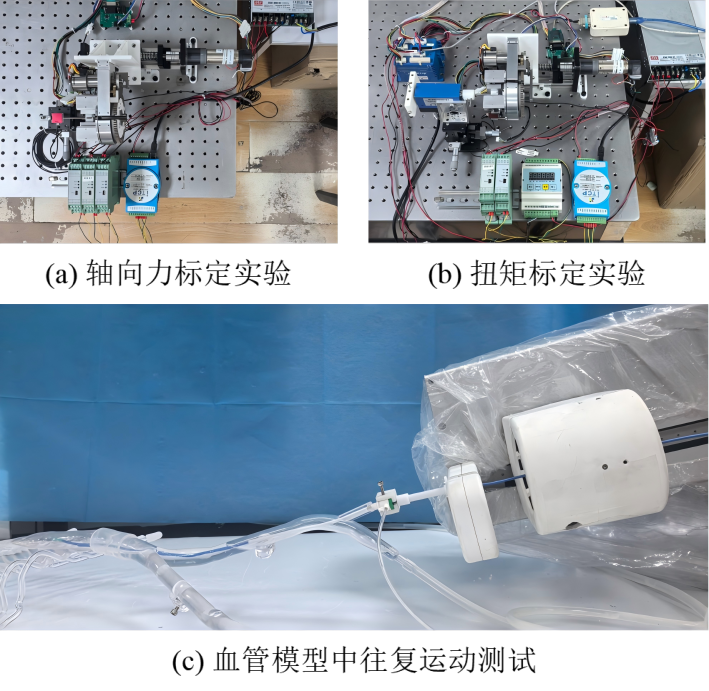
\includegraphics[width=0.88\linewidth]{fig4.png}
	\bicaption{实验设置}{Experimental setup and two test configurations}
	\label{fig4}
\end{figure*}

\subsection{测量参数标定与多阶段承载验证}

在双单元同轴台架上，采用已知砝码载荷和测头标定传递矩阵 $\bm{H}_0$、有效力臂 $R_{\text{eff}}$ 与静态零偏 $\bm{b}$。通过不同恒定速度与角速度的自由空载运动，辨识内侧浮动组件质量 $m_s$、旋转转动惯量 $J_s$ 及摩擦阻尼参数 $c_v$、$c_f$。

在同轴台架上开展多阶段承载验证，适当延长S3与S7的持续时间，分别观测副爪闭合与主爪闭合瞬间的测力跳变。实验表明，当滑台维持静止时，夹爪闭合冲击仅表现为持续约 $15\sim20\,{\rm ms}$ 的高频微小扰动，无宏观载荷转移；当进入S4主爪完全松开及S8副爪释放时，测力通道分别发生阶跃卸载与回弹重加载。测得夹爪单侧硅胶垫综合等效刚度为 $k_M=1.28\,{\rm N}/{\rm mm}$，回弹分配比 $\eta_k=0.74$。

\subsection{对比实验结果与指标分析}

综合对比实验在双单元同轴台架与介入血管模型台架上分别开展，涵盖纯轴向递送与轴向推进伴随周向旋转两种典型工况。对比方法包括：1) 原始未补偿信号（Raw）；2) 传统经验标定与运动学偏置扣除（Kinematic Bias）；3) 纯物理动力学模型（Physics Baseline）；4) 本文提出的物理模型融合GRU残差补偿方法（Physics + GRU）。

\subsubsection{同轴配对参考误差分析}

在同轴台架的配对试次中，以配对不换手试次作为连续递送参考，分别计算稳态递送阶段（S1、S2、S10）与重加载阶段（S9）的均方根误差（RMSE）与平均绝对误差（MAE）：
\begin{align}
	\label{eq17}
	\text{RMSE}_p = \sqrt{\frac{1}{N}\sum_{k=1}^N (w_{\text{fb},p}[k] - w_{\text{ref},p}[k])^2},\quad p \in \{F,\tau\}
\end{align}
式中，$p$ 表示评价通道，$\Omega_s$ 表示对应阶段的样本集合。同时，在包含S3～S9完整的换手全周期窗口内，统计反馈输出相对于换手前目标水平的最大波动峰峰值 $E_{\text{peak}}$，以及重加载后恢复至参考误差带以内所需的恢复时间 $t_{\text{rec}}$：
\begin{align}
	\label{eq18}
	\begin{aligned}
		t_{\text{rec}} &= \inf \Big\{ t > t_{\text{S8,end}} : \left|\frac{F_{\text{fb}}(t') - F_{\text{ref}}(t')}{F_{\text{ref}}(t')}\right| \le 5\%, \\
		&\qquad\quad \forall t' \in [t, t+t_{\text{win}}] \Big\} - t_{\text{S8,end}}
	\end{aligned}
\end{align}
式中，$t_{\text{win}}$ 为重加载恢复时间搜索区间。实验统计结果如表\ref{tab1}所示。

\begin{table*}[h!t]
	\centering
	\bicaption{稳态递送与重加载阶段力反馈重构误差对比}{Comparison of force feedback reconstruction errors during steady delivery and reloading}
	\label{tab1}
	\begin{tabular}{lll}
		\toprule
		递送阶段 / 评价工况 & 评价指标 & 力反馈重构表现 \\
		\midrule
		S1稳态推进（轴向） & 轴向力RMSE / MAE & 待填入具体实验对比指标 \\
		S9重加载阶段（轴向） & 恢复时间 / 波动幅值 & 待填入具体实验对比指标 \\
		复合推进旋转（轴向+扭矩） & 综合重构RMSE ($F$/$\tau$) & 待填入具体实验对比指标 \\
		\bottomrule
	\end{tabular}
\end{table*}

\subsubsection{阻力突变响应评估}

为检验补偿方法在消除换手伪影的同时是否能够真实传递远端新增阻力，开展未训练阻力突变测试。在S1稳态递送中途和S9重加载刚开始时，通过第二操作手在未预告时刻施加阶跃阻力突变。

\begin{figure*}[h!t]
	\centering
	\fbox{\parbox{0.85\linewidth}{\raggedright 【图5占位说明：(a) 同轴台架S1稳态递送阶段的未训练阻力突变响应，绘制原始测力、物理模型、GRU预测与连续参考曲线；(b) S9重加载启动初期的阻力突变响应曲线，展示重加载过渡项与残差网络对突发阻力的快速跟随能力。】}}
	\bicaption{S1与S9阶段未训练阻力突变响应曲线}{Disturbance response waveforms to untrained resistance step in S1 and S9 stages}
	\label{fig5}
\end{figure*}

\subsubsection{消融实验与模型泛化性分析}

进一步开展消融实验与泛化性测试，设置移除重加载过渡项（w/o Reloading Model）及移除GRU残差网络（w/o GRU）两组消融变体。在不同推进速度（$5\,{\rm mm/s}$、$10\,{\rm mm/s}$、$15\,{\rm mm/s}$）与不同夹爪预紧力条件下测试模型的泛化表现。

\begin{figure*}[h!t]
	\centering
	\fbox{\parbox{0.85\linewidth}{\raggedright 【图6占位说明：(a) Physics + GRU、w/o Reloading Model 与 w/o GRU在S9阶段重构误差的消融对比柱状图；(b) 不同推进速度与预紧力工况下力反馈重构RMSE变化趋势图。】}}
	\bicaption{消融实验对比与不同速度及夹持预紧力下的泛化性分析}{Ablation study and generalization performance under various velocities and clamping forces}
	\label{fig6}
\end{figure*}

\subsubsection{血管模型连续递送波形重构}

在具有真实解剖形态的介入血管模型中，操作机器人执行多周期往复夹持长距离连续推进与旋转递送。记录未补偿测力信号与本文方法输出的力与扭矩波形。

\begin{figure*}[h!t]
	\centering
	\fbox{\parbox{0.85\linewidth}{\raggedright 【图7占位说明：(a) 介入血管模型多周期往复推进与旋转递送实测曲线，上栏为轴向反馈力，下栏为周向反馈扭矩；(b) 局部换手重加载窗口放大图，对比原始测量波形与重构连续反馈波形。】}}
	\bicaption{介入血管模型多周期往复递送反馈波形重构}{Reconstructed continuous force and torque feedback waveforms during multi-cycle delivery in vascular phantom}
	\label{fig7}
\end{figure*}

\section{讨论（Discussion）}

实验结果表明，往复夹持机构近端测力波动的核心诱因在于交接过程中的弹性载荷亏缺与浮动组件运动惯性。本文提出的物理模型结合GRU残差补偿方法，在机理明确的惯性、摩擦与弹性恢复阶段由物理模型提供确定性基准，而在微滑移与接触迟滞显著的复杂过渡区由数据驱动网络进行动态残差修正。二者的有效结合既保证了补偿算法的物理可解释性与对未训练突发外载的即时响应能力，又克服了纯解析模型对接触刚度非线性难以精确标定的缺陷。

\section{结论（Conclusions）}

本文针对往复夹持式血管介入机器人近端测力通道中的换手波动与机构运动干扰问题，提出了融合多阶段接触力学模型与GRU时序残差网络的连续力反馈重构方法。研究建立了涵盖正常递送、双爪共持与重加载过程的动力学和串联接触刚度模型，推导了轴向与周向耦合的等效恢复行程与显式重加载过渡项。搭建了双单元同轴参考台架与介入血管模型实验平台，以不换手真实载荷为参考进行了定量评价与消融实验。结果表明，所提方法有效抑制了换手冲击与重加载迟滞，重构出连续平滑的主端力反馈，并保留了对血管突发阻力的实时响应能力，为往复夹持介入机器人的力触觉高保真再现提供了有效途径。

\noindent
\textbf{数据可用性声明}

支撑本研究的科学数据已在中国科学院科学数据银行（Science Data Bank）ScienceDB 平台公开发布，访问地址为~\url{https://www.scidb.cn/surl/robot}。

% -------- 参考文献表（支持 Zotero 导出 references.bib）
\nocite{*}
\bibliographystyle{jqr-num}
\bibliography{references}

\begin{AuthorIntroduction}
\Intro 第一作者：隋凯丞（2000--），男，博士研究生。研究领域：血管介入手术机器人，机器人力感知与控制。E-mail: suikaicheng24@mails.ucas.ac.cn。
\Intro 通信作者：刘浩（1976--），男，博士，研究员，博士生导师。研究领域：医疗微创手术机器人，智能控制。E-mail: liuhao@sia.cn。
\end{AuthorIntroduction}

\balance
\end{document}
